\section{Решение начально-краевой задачи для дифференциальных уравнений в частных производных гиперболического типа}

\subsection{Постановка задачи}
Используя явную и неявную конечно-разностные схемы, решить начально-краевую задачу для дифференциального уравнения гиперболического типа. Аппроксимацию второго начального условия произвести с первым и со вторым порядком. Осуществить реализацию трех вариантов аппроксимации граничных условий, содержащих производные: двухточечная аппроксимация с первым порядком, трехточечная аппроксимация со вторым порядком, двухточечная аппроксимация со вторым порядком. В различные моменты времени вычислить погрешность численного решения путем сравнения результатов с приведенным в задании аналитическим решением $U(x, t)$. Исследовать зависимость погрешности от сеточных параметров $\tau$, $h$.

{\bfseries Вариант:} 2
\begin{align*}
& \frac{\partial^2 u}{\partial t^2} = a^2 \frac{\partial^2 u}{\partial x^2},\ a^2 > 0 \\
& u_x(0, t) - u(0, t) = 0 \\
& u_x(\pi, t) - u(\pi, t) = 0 \\
& u(x, 0) = \sin x + \cos x \\
& u_t(x, 0) = -a(\sin x + \cos x) \\
& U(x, t) = \sin(x - at) + \cos(x + at) \\
\end{align*}
\pagebreak

\subsection{Результаты работы}
\begin{figure}[h!]
\centering
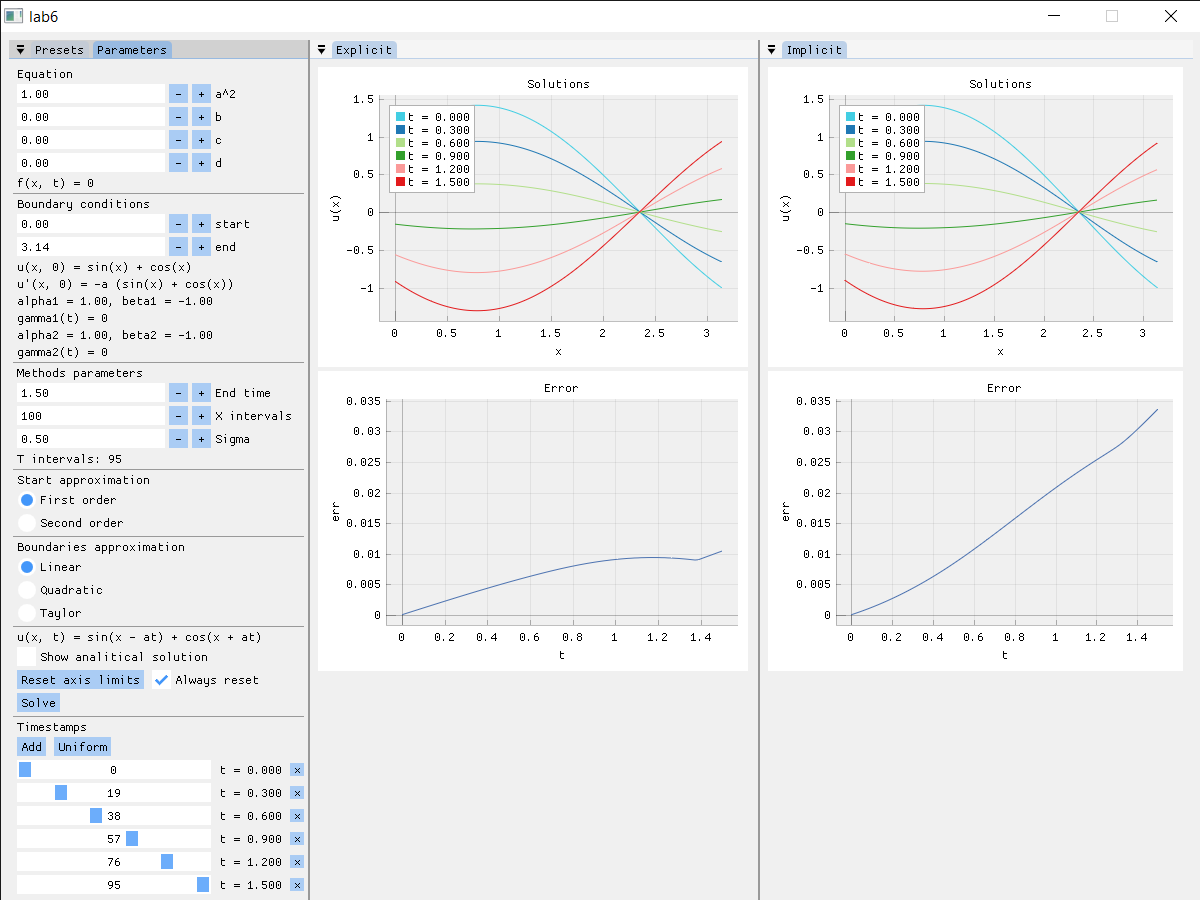
\includegraphics[height=.4\textheight]{lab6_linear}
\caption{Решение с аппроксимацией граничных и начальных условий с первым порядком}
\end{figure}

\vfill

\begin{figure}[h!]
\centering
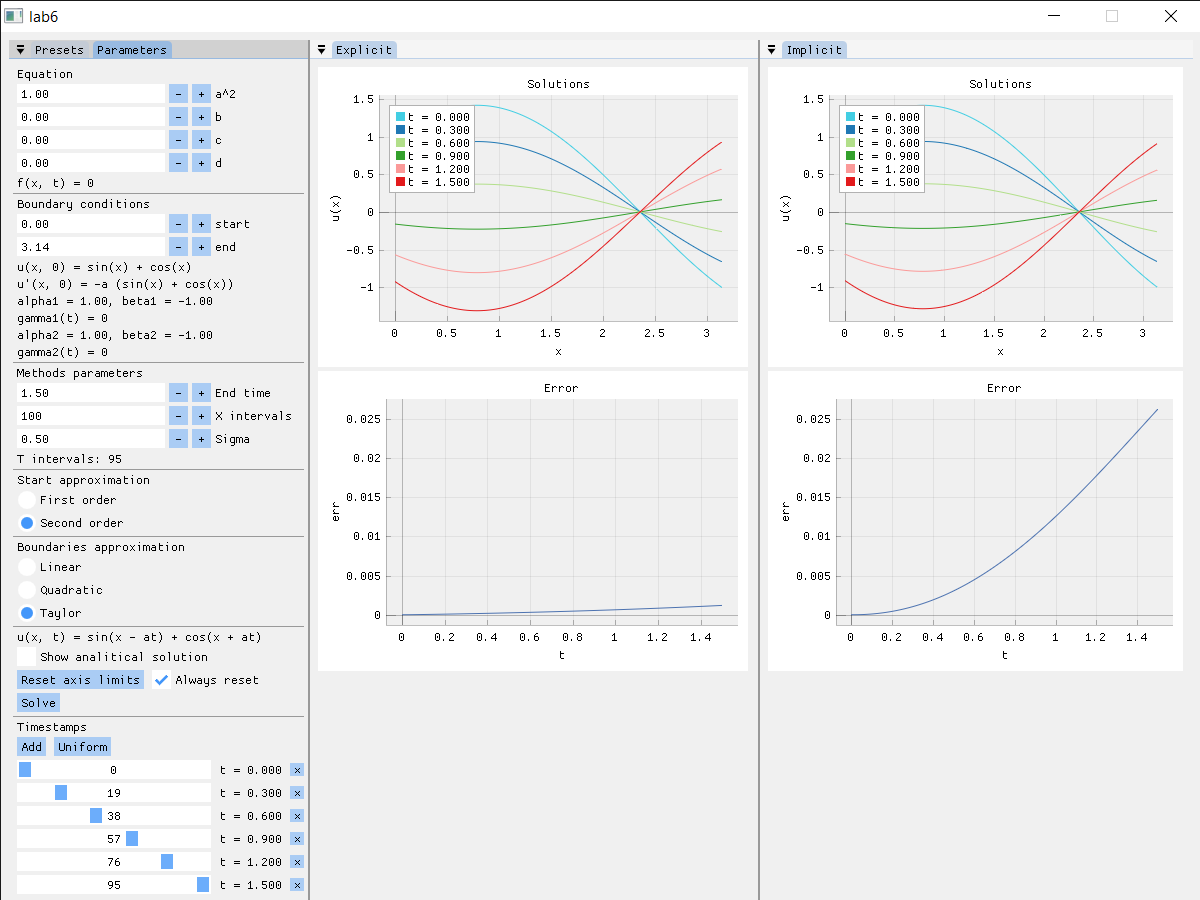
\includegraphics[height=.4\textheight]{lab6_taylor}
\caption{Решение с аппроксимацией граничных и начальных условий со вторым порядком}
\end{figure}
\pagebreak

\subsection{Исходный код}
\lstinputlisting{../../include/partial_differential/hyperbolic_pde.hpp}
\pagebreak
